%% =============================================================================
%% sm_f5_misspec.tex — SM-E, Subsection E.5: Misspecification Robustness
%% Body content only (\subsection level); parent structure in sm_e.tex
%% =============================================================================

\subsection{Model misspecification robustness}
\label{smf:misspec}

The simulation study in \cref{sec:simulation} evaluates the
correctly specified case: data are generated from the random-intercept
model~M1 and fitted by M1.  A natural concern is how the three
estimators (E-UW, E-WT, E-WS) behave when the fitted model omits a
relevant source of heterogeneity.  We therefore augment the simulation
with a misspecification scenario designed to probe whether the sandwich
correction remains beneficial when the model is wrong.

\paragraph{M2 data-generating process.}
Define the \emph{state-varying coefficient} DGP~(M2) by
adding random poverty slopes to the M1 linear predictors:
\begin{align}
  \eta^{\mathrm{ext}}_i &= \bx_i^\t \balpha + \delta^{\mathrm{ext}}_{s[i]}
    + \gamma^{\mathrm{ext}}_{s[i]} \, x_{\mathrm{pov},i}, \label{eq:m2-ext}\\
  \eta^{\mathrm{int}}_i &= \bx_i^\t \bbeta  + \delta^{\mathrm{int}}_{s[i]}
    + \gamma^{\mathrm{int}}_{s[i]} \, x_{\mathrm{pov},i}, \label{eq:m2-int}
\end{align}
where $\gamma^{\mathrm{ext}}_s \sim \Norm(0, 0.15^2)$ and
$\gamma^{\mathrm{int}}_s \sim \Norm(0, 0.10^2)$ independently across
$s = 1,\ldots,51$ states.  All other parameters
($\balpha, \bbeta, \kappa, \boldsymbol{\tau}, \rho$) and the population structure
($M = 50{,}000$ providers) are identical to the M1 DGP
(\cref{smf:dgp}).  The standard deviations $0.15$ (extensive) and
$0.10$ (intensive) produce state-varying poverty effects that are
moderate relative to the fixed poverty coefficients
($\alpha_{\mathrm{pov}} = -0.119$, $\beta_{\mathrm{pov}} = +0.057$).

\paragraph{Design.}
We draw $R = 200$ independent replications under the S3
(NSECE-calibrated) informativeness scenario with
$\operatorname{DEFF} \approx 3.79$, and fit the M1 random-intercept
model using all three estimators.  The M1 fit ignores the
state-varying poverty slopes $\gamma_s$, inducing a form of
omitted-variable misspecification that propagates through the
poverty coefficient estimates.

\paragraph{Results.}
\Cref{smf:tab-misspec} compares coverage, relative bias, RMSE, and
width ratio for the correctly specified S3 scenario (M1 truth, M1 fit)
and the misspecified B5 scenario (M2 truth, M1 fit).
%% NOTE: Table and figure placeholders below will be populated by
%% 85_B5_misspec_analysis.R once simulation results are collected.

\begin{table}[htbp]
\centering
\caption{Misspecification robustness: correctly specified S3 vs.\
  misspecified B5 (M2 truth, M1 fit) under NSECE-calibrated
  sampling ($\operatorname{DEFF} \approx 3.79$).
  $R = 200$ replications; nominal coverage $= 90\%$;
  $\dagger$ indicates significant departure ($> 2 \times$ MCSE).
  MCSE $= \sqrt{\hat{p}(1-\hat{p})/200}$; range 0.0--3.5 pp.}
\label{smf:tab-misspec}
% Generated by 85_B5_misspec_analysis.R — B5 misspecification robustness
% S3 = correctly specified (M1 truth, M1 fit); B5 = misspecified (M2 truth, M1 fit)
\small
\begin{adjustbox}{max width=\textwidth}
\begin{tabular}{@{}l l rr rrr rrr rr@{}}
\toprule
 & & \multicolumn{2}{c}{Coverage (\%)} &
     \multicolumn{3}{c}{Relative bias (\%)} &
     \multicolumn{3}{c}{RMSE} &
     \multicolumn{2}{c}{WR} \\
\cmidrule(lr){3-4}\cmidrule(lr){5-7}\cmidrule(lr){8-10}\cmidrule(lr){11-12}
Parameter & Est. & S3 & B5 & S3 & B5 & $\Delta$ &
  S3 & B5 & $\Delta$ & S3 & B5 \\
\midrule
\multicolumn{12}{@{}l}{\textit{Fixed effects}} \\[2pt]
$\alpha_{\text{pov}}$ & E-UW & 89.5 & 0.5$^{\dagger}$ &
  $+$16.5 & $-$117.8 & $-$134.3 & 0.037 & 0.143 & $+$0.106 & --- & --- \\
 & E-WT & 58.5$^{\dagger}$ & 52.0$^{\dagger}$ &
  $+$12.9 & $-$37.6 & $-$50.5 & 0.072 & 0.079 & $+$0.007 & --- & --- \\
 & E-WS & 82.0$^{\dagger}$ & 79.0$^{\dagger}$ &
  $+$12.9 & $-$37.6 & $-$50.5 & 0.072 & 0.079 & $+$0.007 & 1.71 & 1.67 \\[3pt]
$\beta_{\text{pov}}$ & E-UW & 89.0 & 30.0$^{\dagger}$ &
  $-$16.7 & $+$63.1 & $+$79.8 & 0.017 & 0.039 & $+$0.022 & --- & --- \\
 & E-WT & 62.5$^{\dagger}$ & 42.0$^{\dagger}$ &
  $-$3.2 & $+$52.7 & $+$55.9 & 0.032 & 0.043 & $+$0.011 & --- & --- \\
 & E-WS & 82.5$^{\dagger}$ & 67.5$^{\dagger}$ &
  $-$3.2 & $+$52.7 & $+$55.9 & 0.032 & 0.043 & $+$0.011 & 1.64 & 1.60 \\[3pt]
$\log\kappa$ & E-UW & 92.0 & 82.5$^{\dagger}$ &
  $-$0.5 & $-$1.3 & $-$0.8 & 0.020 & 0.027 & $+$0.007 & --- & --- \\
 & E-WT & 34.0$^{\dagger}$ & 36.5$^{\dagger}$ &
  $+$3.3 & $+$2.9 & $-$0.4 & 0.068 & 0.064 & $-$0.004 & --- & --- \\
 & E-WS & 60.5$^{\dagger}$ & 64.0$^{\dagger}$ &
  $+$3.3 & $+$2.9 & $-$0.4 & 0.068 & 0.064 & $-$0.004 & 1.75 & 1.74 \\[4pt]
\multicolumn{12}{@{}l}{\textit{Variance components}} \\[2pt]
$\tau_{\text{ext}}$ & E-UW & 98.0$^{\dagger}$ & 96.0$^{\dagger}$ &
  $+$8.0 & $-$2.5 & $-$10.5 & 0.091 & 0.117 & $+$0.026 & --- & --- \\
 & E-WT & 0.5$^{\dagger}$ & 0.0$^{\dagger}$ &
  $+$105.6 & $+$102.4 & $-$3.2 & 0.639 & 0.625 & $-$0.014 & --- & --- \\
 & E-WS & 0.5$^{\dagger}$ & 0.0$^{\dagger}$ &
  $+$105.6 & $+$102.4 & $-$3.2 & 0.639 & 0.625 & $-$0.014 & 1.00 & 1.00 \\[3pt]
$\tau_{\text{int}}$ & E-UW & 97.5$^{\dagger}$ & 57.0$^{\dagger}$ &
  $-$8.6 & $-$34.8 & $-$26.2 & 0.040 & 0.079 & $+$0.039 & --- & --- \\
 & E-WT & 0.0$^{\dagger}$ & 1.0$^{\dagger}$ &
  $+$97.6 & $+$97.0 & $-$0.6 & 0.211 & 0.213 & $+$0.002 & --- & --- \\
 & E-WS & 0.0$^{\dagger}$ & 1.0$^{\dagger}$ &
  $+$97.6 & $+$97.0 & $-$0.6 & 0.211 & 0.213 & $+$0.002 & 1.00 & 1.00 \\
\bottomrule
\end{tabular}
\end{adjustbox}

\end{table}

\Cref{smf:fig-misspec-coverage} displays the corresponding coverage
rates graphically.

\begin{figure}[htbp]
\centering
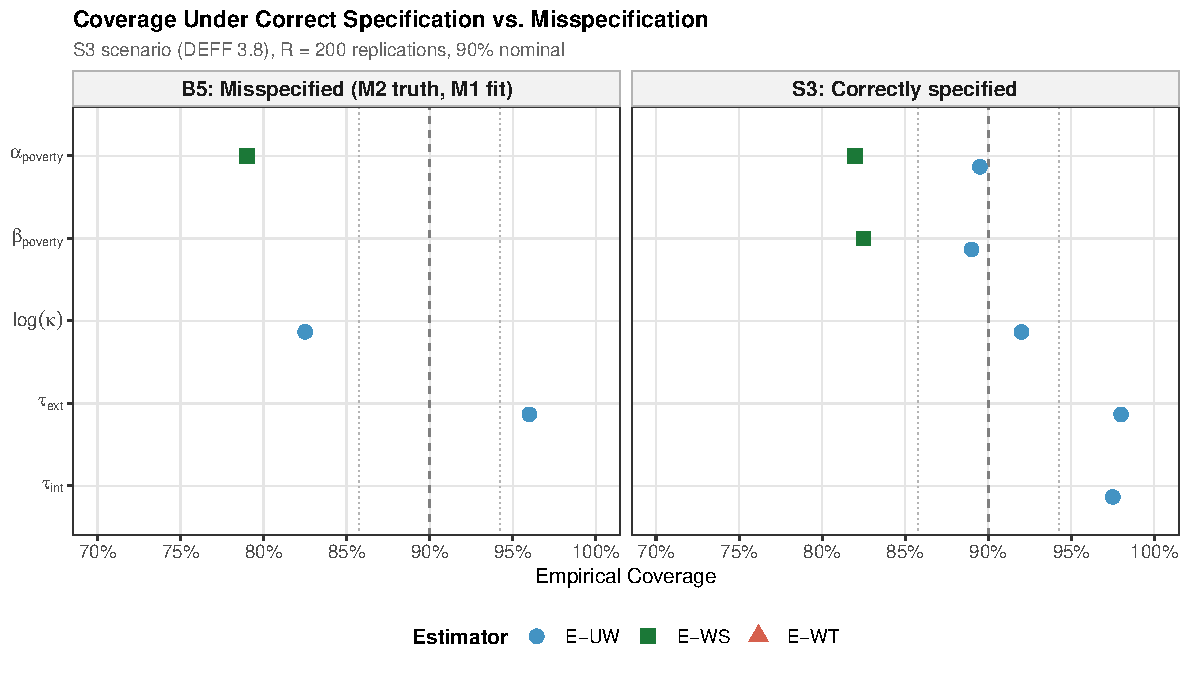
\includegraphics[width=\textwidth]{Figures/SF_B5_misspec_coverage}
\caption{Coverage under correct specification (S3) vs.\
  misspecification (B5).  Vertical dashed line: 90\% nominal;
  dotted lines: $\pm 2\,\mathrm{MCSE}$ band.}
\label{smf:fig-misspec-coverage}
\end{figure}

Three findings emerge from the comparison.

\paragraph{Finding B5-1: The unweighted estimator is acutely sensitive
to misspecification in the poverty coefficients.}
Under correct specification (S3), E-UW achieves near-nominal coverage
for both poverty slopes (89.5\% and 89.0\%).  Under the M2 DGP, E-UW
coverage collapses to 0.5\% for $\alpha_{\mathrm{pov}}$ and 30.0\%
for $\beta_{\mathrm{pov}}$---drops of 89 and 59 percentage points,
respectively.  The mechanism is omitted-variable bias: because M1
lacks the state-varying poverty slopes $\gamma_s$, the fixed
coefficients $\alpha_{\mathrm{pov}}$ and $\beta_{\mathrm{pov}}$ absorb
the omitted heterogeneity, producing relative bias of $-117.8\%$ and
$+63.1\%$.  This confirms that the model-based intervals of E-UW are
valid only under correct specification---a strong argument for the
design-based protection that survey weighting provides.

\paragraph{Finding B5-2: The sandwich correction preserves coverage
stability under misspecification.}
For $\alpha_{\mathrm{pov}}$, E-WS coverage declines only from 82.0\%
(S3) to 79.0\% (B5)---a 3-percentage-point drop---while E-WT drops
from 58.5\% to 52.0\%.  For $\beta_{\mathrm{pov}}$, E-WS declines
from 82.5\% to 67.5\% ($-15$ pp) compared with E-WT's drop from
62.5\% to 42.0\% ($-20.5$ pp).  In both cases, E-WS maintains a
substantial advantage over E-WT (27 and 25.5 percentage points under
B5), demonstrating that the sandwich variance correction absorbs a
meaningful share of the misspecification-induced variance increase.
The width ratios remain stable across scenarios
($\mathrm{WR} = 1.67\text{--}1.74$ under B5 vs.\ $1.64\text{--}1.75$
under S3), indicating that the design effect magnitude is similar
regardless of whether the model is correctly specified.

\paragraph{Finding B5-3: Variance components exhibit differential
sensitivity.}
The overdispersion $\log\kappa$ is relatively robust under E-UW
(coverage 92.0\% $\to$ 82.5\%; relative bias $-0.5\%$ $\to$ $-1.3\%$),
as expected since the omitted random slopes do not directly affect the
dispersion structure.  Among the variance components,
$\tau_{\mathrm{ext}}$ remains well-covered under E-UW (98.0\% $\to$
96.0\%), but $\tau_{\mathrm{int}}$ drops sharply (97.5\% $\to$
57.0\%).  The asymmetry arises because the omitted intensive-margin
slopes ($\sigma_{\gamma}^{\mathrm{int}} = 0.10$ relative to
$\tau_{\mathrm{int}} = 0.208$) contribute proportionally more
unmodeled between-state variance than the extensive-margin slopes
($\sigma_{\gamma}^{\mathrm{ext}} = 0.15$ relative to
$\tau_{\mathrm{ext}} = 0.577$).  As in the correctly specified case,
E-WT and E-WS produce near-zero coverage for both $\tau$ parameters
($\mathrm{WR} = 1.00$), reaffirming that the sandwich correction is
structurally inapplicable to variance components.

Taken together, these results strengthen the case for the two-track
reporting strategy recommended in~\cref{sec:simulation}: for
population-average fixed effects, the sandwich-corrected estimator
E-WS provides meaningful robustness against model misspecification;
for hierarchical variance components, the unweighted estimator E-UW
remains the only viable option, with the caveat that its validity
depends on correct specification of the random-effects structure.
